\begin{frame}
	\frametitle{Assignment 4}
	\begin{itemize}
		\item Classification of data sets \texttt{image}, \texttt{ringnorm}, \texttt{flare-solar}, \texttt{banana} and \texttt{diabetes} using \texttt{cv}
		\item Cross-validation: \texttt{nfolds = 10} and \texttt{nrepetitions = 5}
		\item Parameter ranges:
	\end{itemize}
	\begin{table}
		\centering
		\begin{tabular}{lll}
			Kernel & Kernel parameter & Regularization\\
			\hline
			linear & $[0]$ & \texttt{np.logspace(-2,2,10)} \\
			polynomial & \texttt{np.arange(1,10)} & \texttt{np.logspace(-2,2,10)}\\
			gaussian & \texttt{np.logspace(-2,2,10)} & \texttt{np.logspace(-2,2,10)}
		\end{tabular}
	\end{table}
	
	\begin{itemize}
		\item KRR with LOOCV $\Rightarrow$ regularization set to \texttt{[0]}
	\end{itemize}
\end{frame}

\begin{frame}
	\frametitle{ROC-Curves \texttt{banana}}
	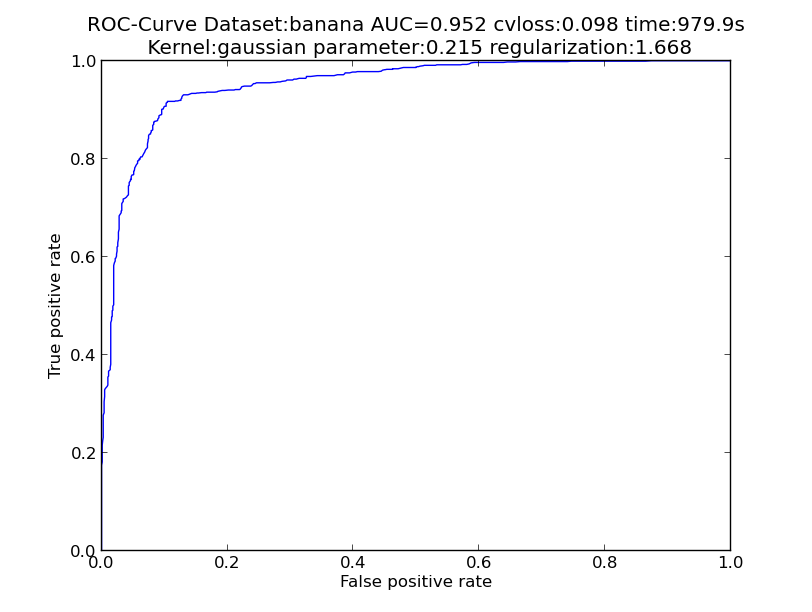
\includegraphics[width=5.5cm]{../report/images/banana.png}
	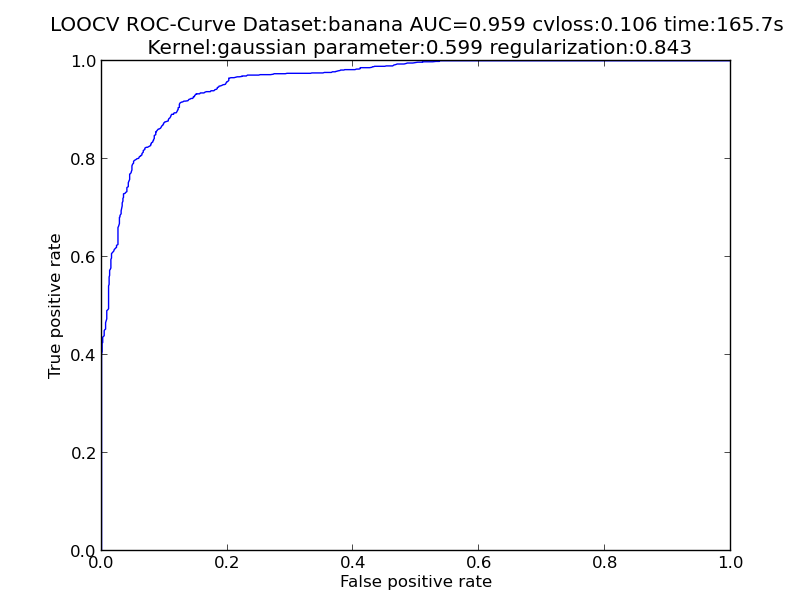
\includegraphics[width=5.5cm]{../report/images/bananaLOOCV.png}
\end{frame}

\begin{frame}
	\frametitle{ROC-Curves \texttt{ringnorm}}
	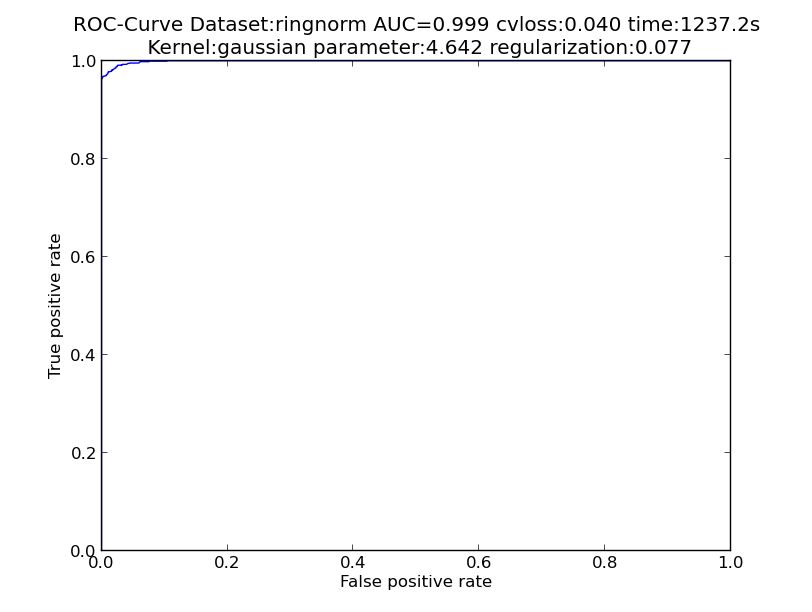
\includegraphics[width=5.5cm]{../report/images/ringnorm.png}
	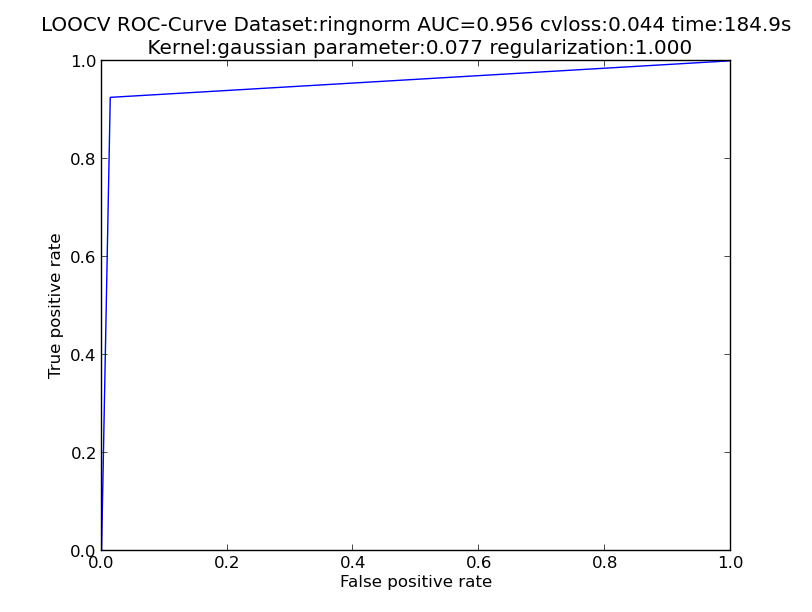
\includegraphics[width=5.5cm]{../report/images/ringnormLOOCV.png}
\end{frame}

\begin{frame}
	\frametitle{ROC-Curves \texttt{image}}
	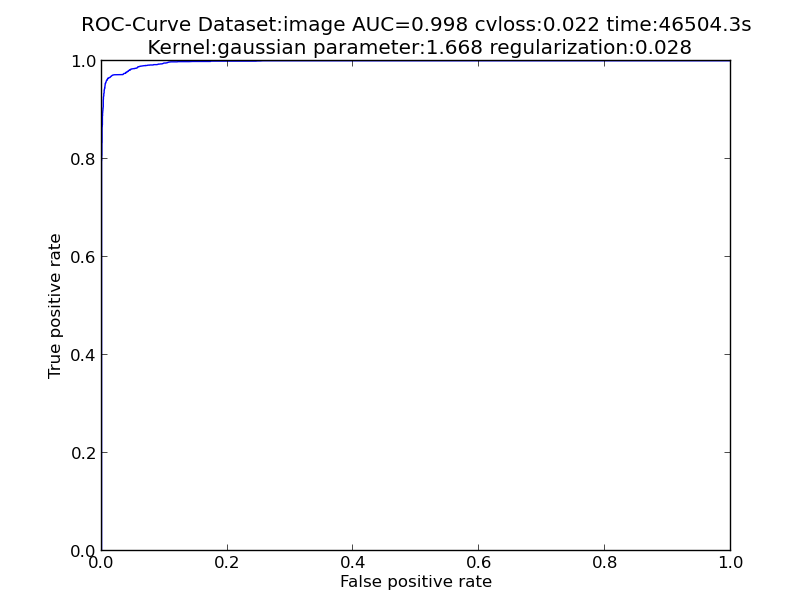
\includegraphics[width=5.5cm]{../report/images/image.png}
	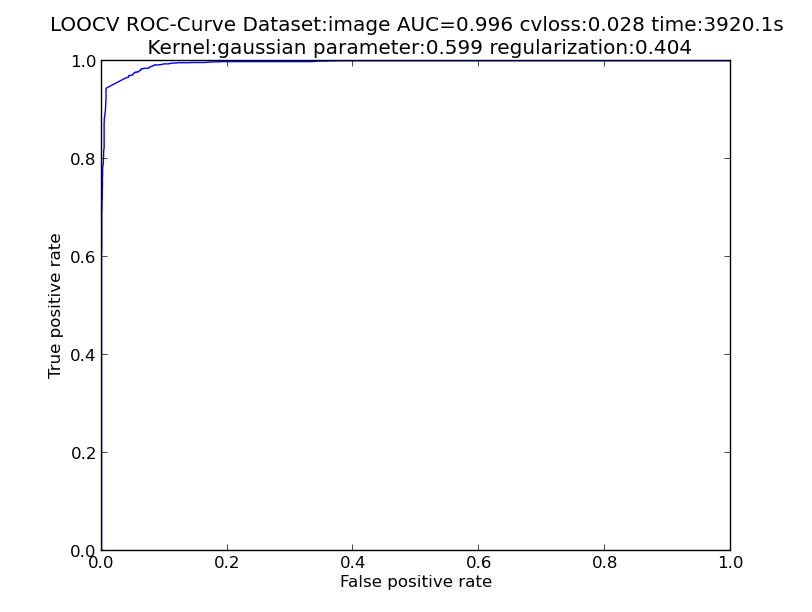
\includegraphics[width=5.5cm]{../report/images/imageLOOCV.png}
\end{frame}

\begin{frame}
	\frametitle{ROC-Curves \texttt{diabetes}}
	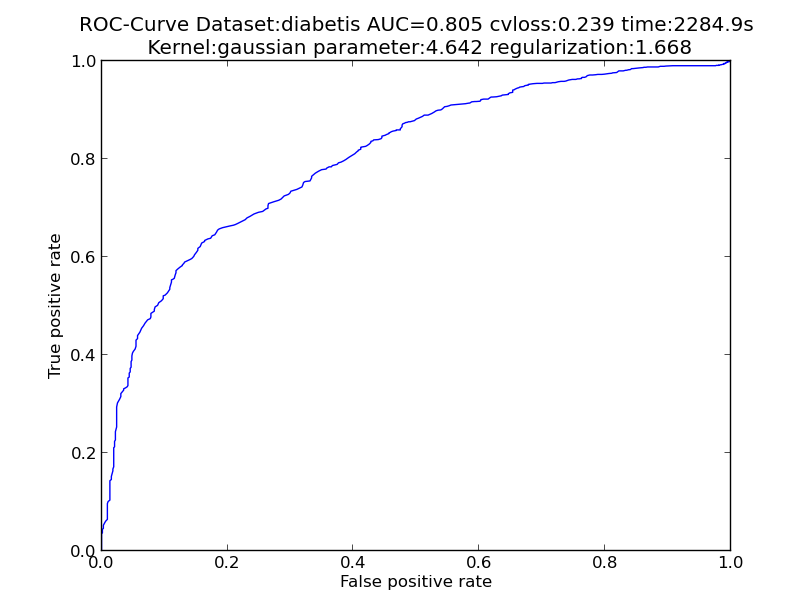
\includegraphics[width=5.5cm]{../report/images/diabetis.png}
	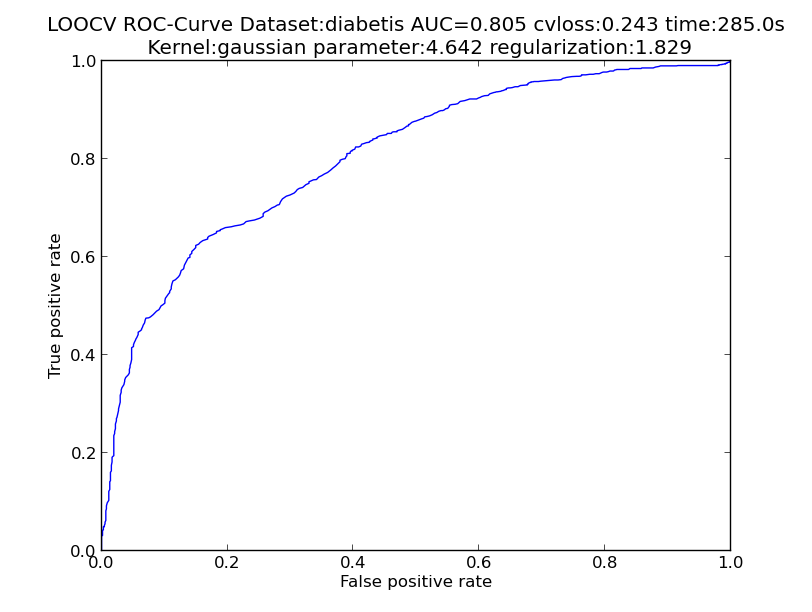
\includegraphics[width=5.5cm]{../report/images/diabetisLOOCV.png}
\end{frame}

\begin{frame}
	\frametitle{ROC-Curves \texttt{flare-solar}}
	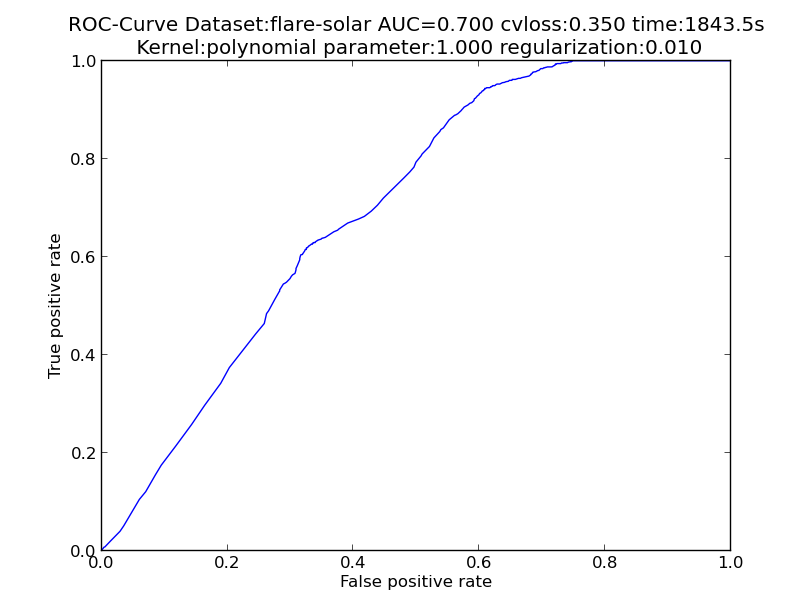
\includegraphics[width=5.5cm]{../report/images/flaresolar.png}
	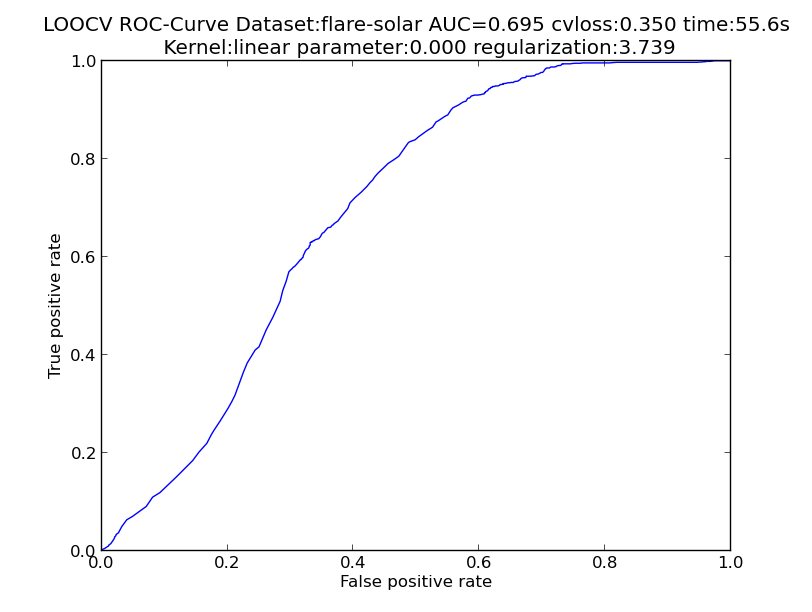
\includegraphics[width=5.5cm]{../report/images/flaresolarLOOCV.png}
\end{frame}

\begin{frame}
	\frametitle{\texttt{banana} in detail}
	\begin{center}
		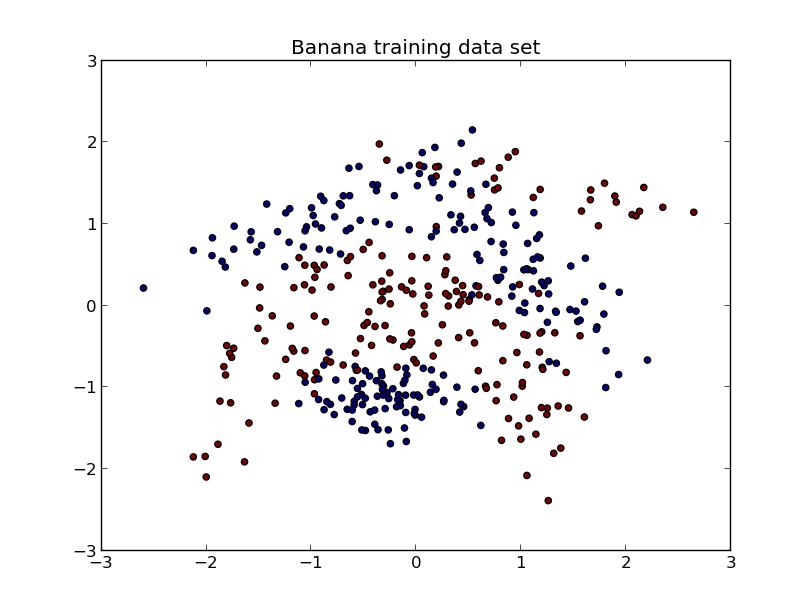
\includegraphics[width=4.5cm]{images/banana_training.png}
		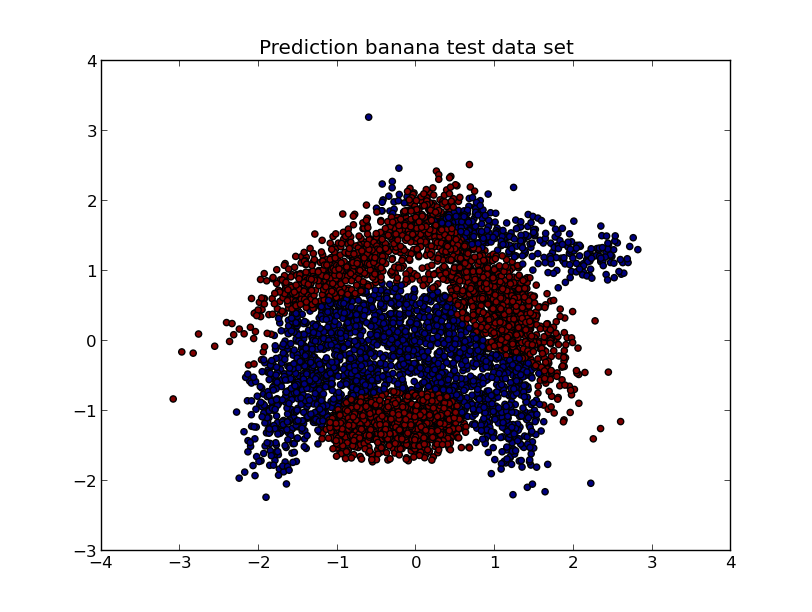
\includegraphics[width=4.5cm]{images/banana_prediction.png}
		\\
		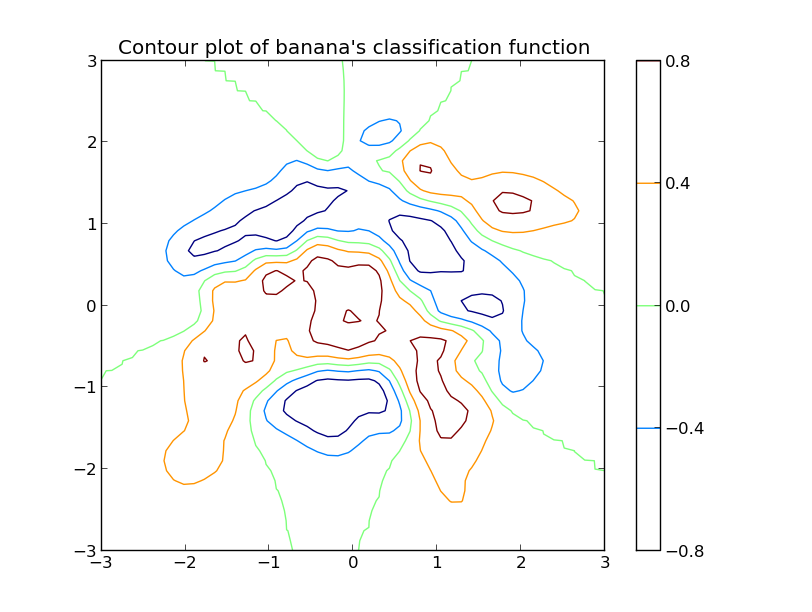
\includegraphics[width=5cm]{images/banana_function.png}
	\end{center}
\end{frame}

\begin{frame}
	\small
	\frametitle{Cross-validation results}
	\begin{table}
		\centering
		\caption{Normal \texttt{cv}}
		\begin{tabular}{llllll}
		Data set& cv loss & AUC & Kernel & Parameter& Regularization\\
		\hline
		image & $0.0225$ & $0.998$ & Gaussian & $1.6681$& $0.0278$\\
		ringnorm & $0.0395$& $0.999$ &Gaussian & $4.6416$& $0.0774$\\
		flare-solar & $0.3499$& $0.7$& polynomial& $1$ & $0.01$\\
		banana & $0.0985$& $0.952$& Gaussian & $0.2154$ & $1.6681$\\
		diabetes & $0.2385$ & $0.805$ & Gaussian& $4.6416$& $1.6681$
		\end{tabular}
	\end{table}
	
	\begin{table}
		\centering
		\caption{LOOCV}
		\begin{tabular}{llllll}
		Data set& cv loss& AUC & Kernel & Parameter& Regularization\\
		\hline
		image & $0.0283$& $0.996$ & Gaussian & $0.5995$& $0.4043$\\
		ringnorm & $0.0475$& $0.956$ & Gaussian & $0.0774$& $1.0$\\
		flare-solar & $0.3505$& $0.695$& linear&  & $3.7391$\\
		banana & $0.106$& $0.959$ & Gaussian & $0.5995$ & $0.8431$\\
		diabetes & $0.2431$ &  $0.805$ & Gaussian& $4.6416$& $1.8293$
		\end{tabular}
		
	\end{table}
\end{frame}

\begin{frame}
	\frametitle{Accuracy comparison}
	\begin{itemize}
		\item Reference loss taken from Machine Learning 2 lecture
		\item Normal \texttt{cv} slightly better than LOOCV
	\end{itemize}
	\begin{table}
		\centering
		\begin{tabular}{llll}
			Data set & cv loss & cv loss LOOCV & reference loss\\
			\hline
			image & $0.0225$ & $0.0283$ & $0.028$\\
			ringnorm & $0.0395$ & $0.0475$ & $0.047$ \\
			flare-solar & $0.3499$ & $0.3505$ & $0.341$\\
			banana & $0.0985$ & $0.106$ & $0.106$ \\
			diabetes & $0.2385$ & $0.2431$ & $0.232$
		\end{tabular}
	\end{table}
\end{frame}

\begin{frame}
	\frametitle{Runtime comparison}
	\begin{itemize}
		\item Speed-up between $6-12$
		\item \texttt{flare-solar} data set is an outlier
		\item Linear kernel has fewer parameter values
	\end{itemize}
	\begin{table}
		\centering
		\begin{tabular}{llll}
		Data set & \texttt{cv} in s & \texttt{cv} with LOOCV in s & speed-up\\
		\hline
		image & $46504$ & $3920$ & $11.9$\\
		ringnorm & $1237$ & $185$ & $6.7$\\
		flare-solar & $1843$ & $56$ & $33$ \\
		banana & $980$ & $166$ & $6$\\
		diabetes & $2284$ & $285$ & $8$
		\end{tabular}
	\end{table}	
\end{frame}

\begin{frame}
	\frametitle{Comparison test data set}
	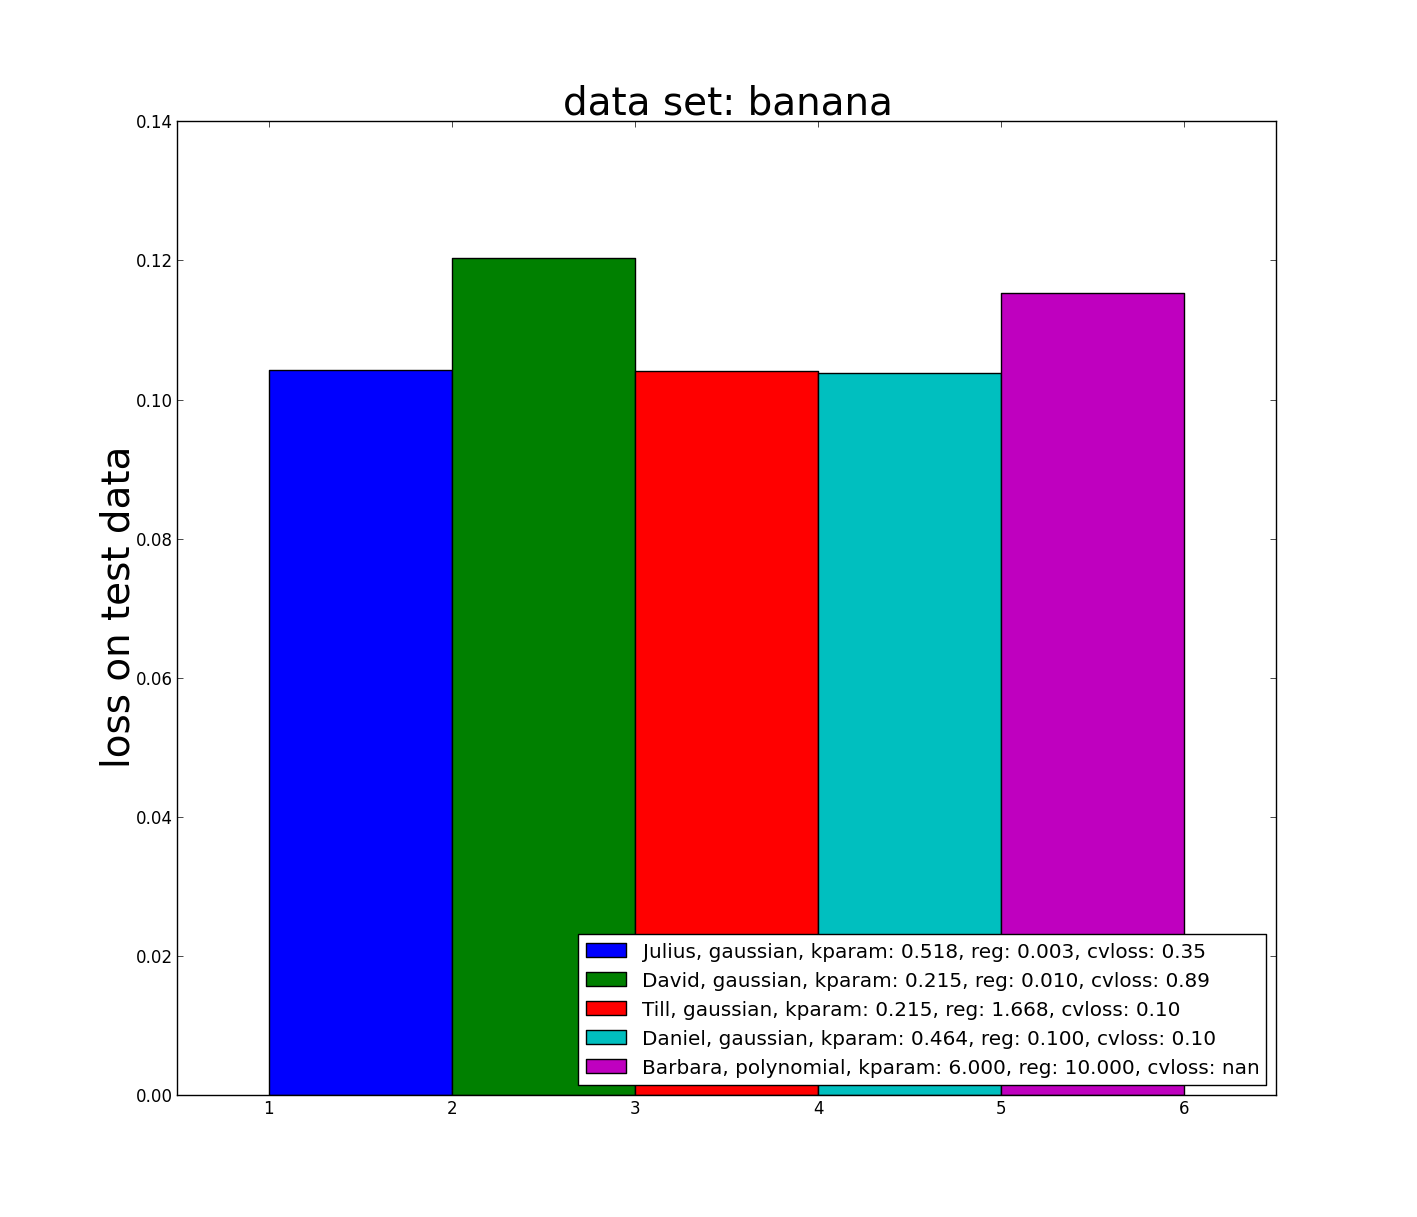
\includegraphics[width=5.75cm]{images/ps3_results_banana.png}
	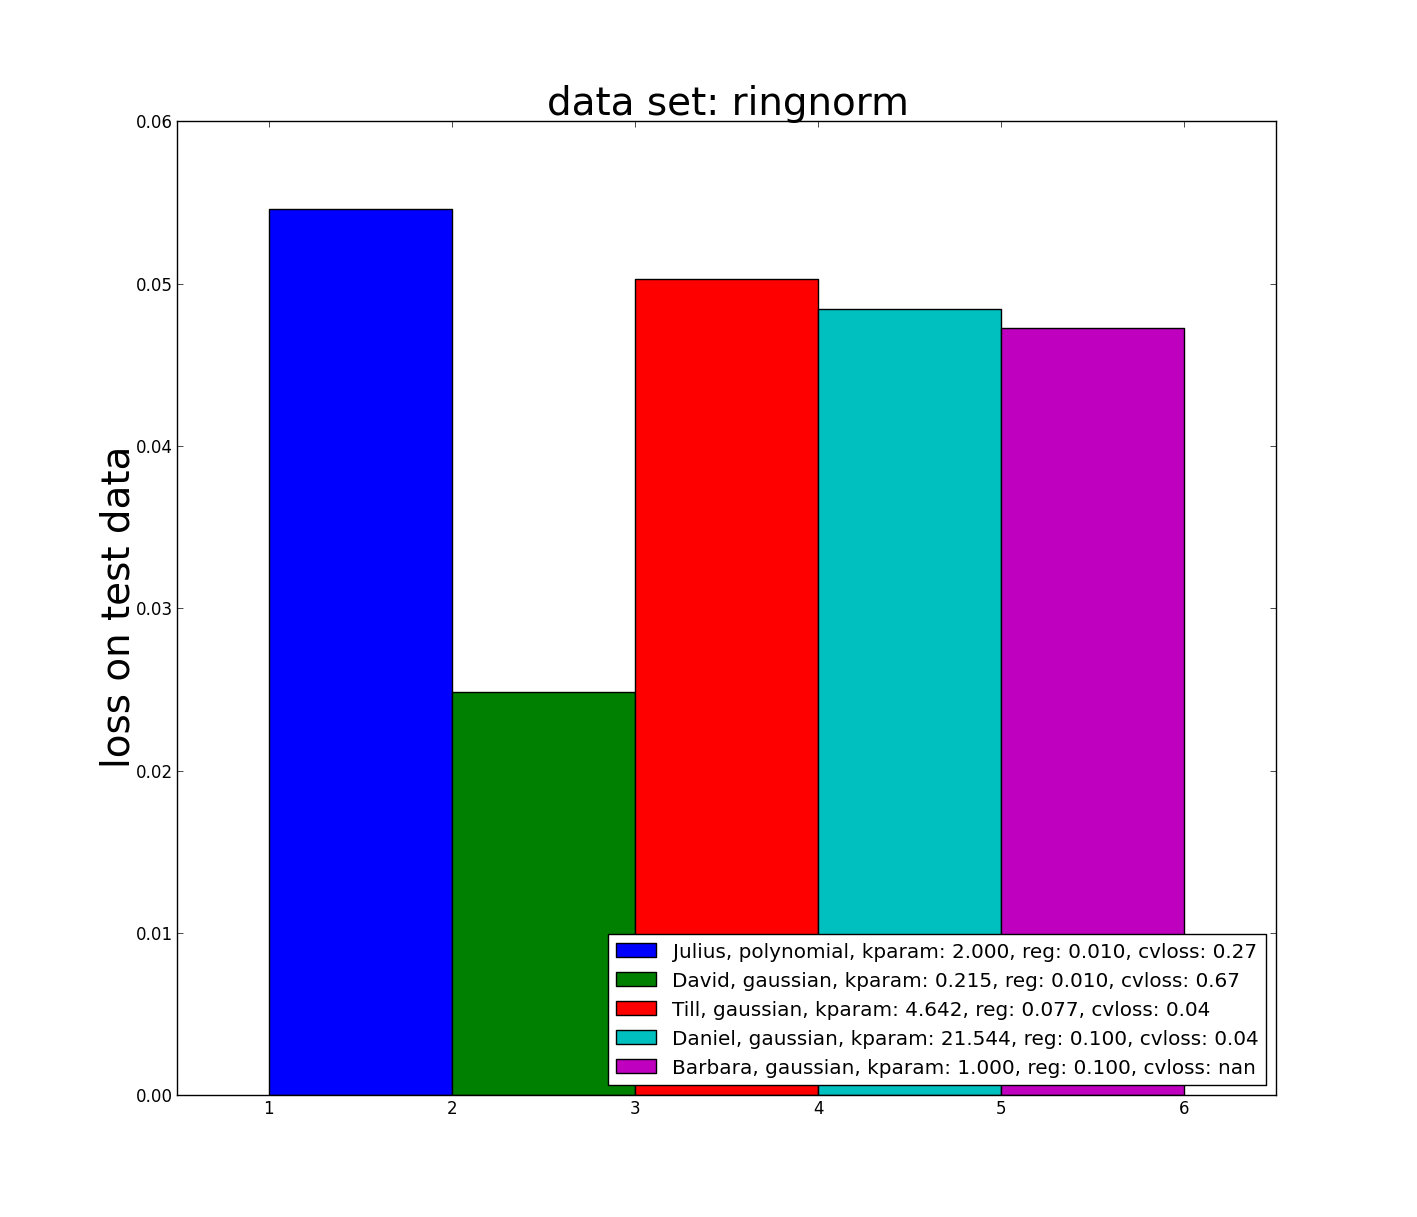
\includegraphics[width=5.75cm]{images/ps3_results_ringnorm.png}
\end{frame}

\begin{frame}
	\frametitle{Comparison test data set contd.}
	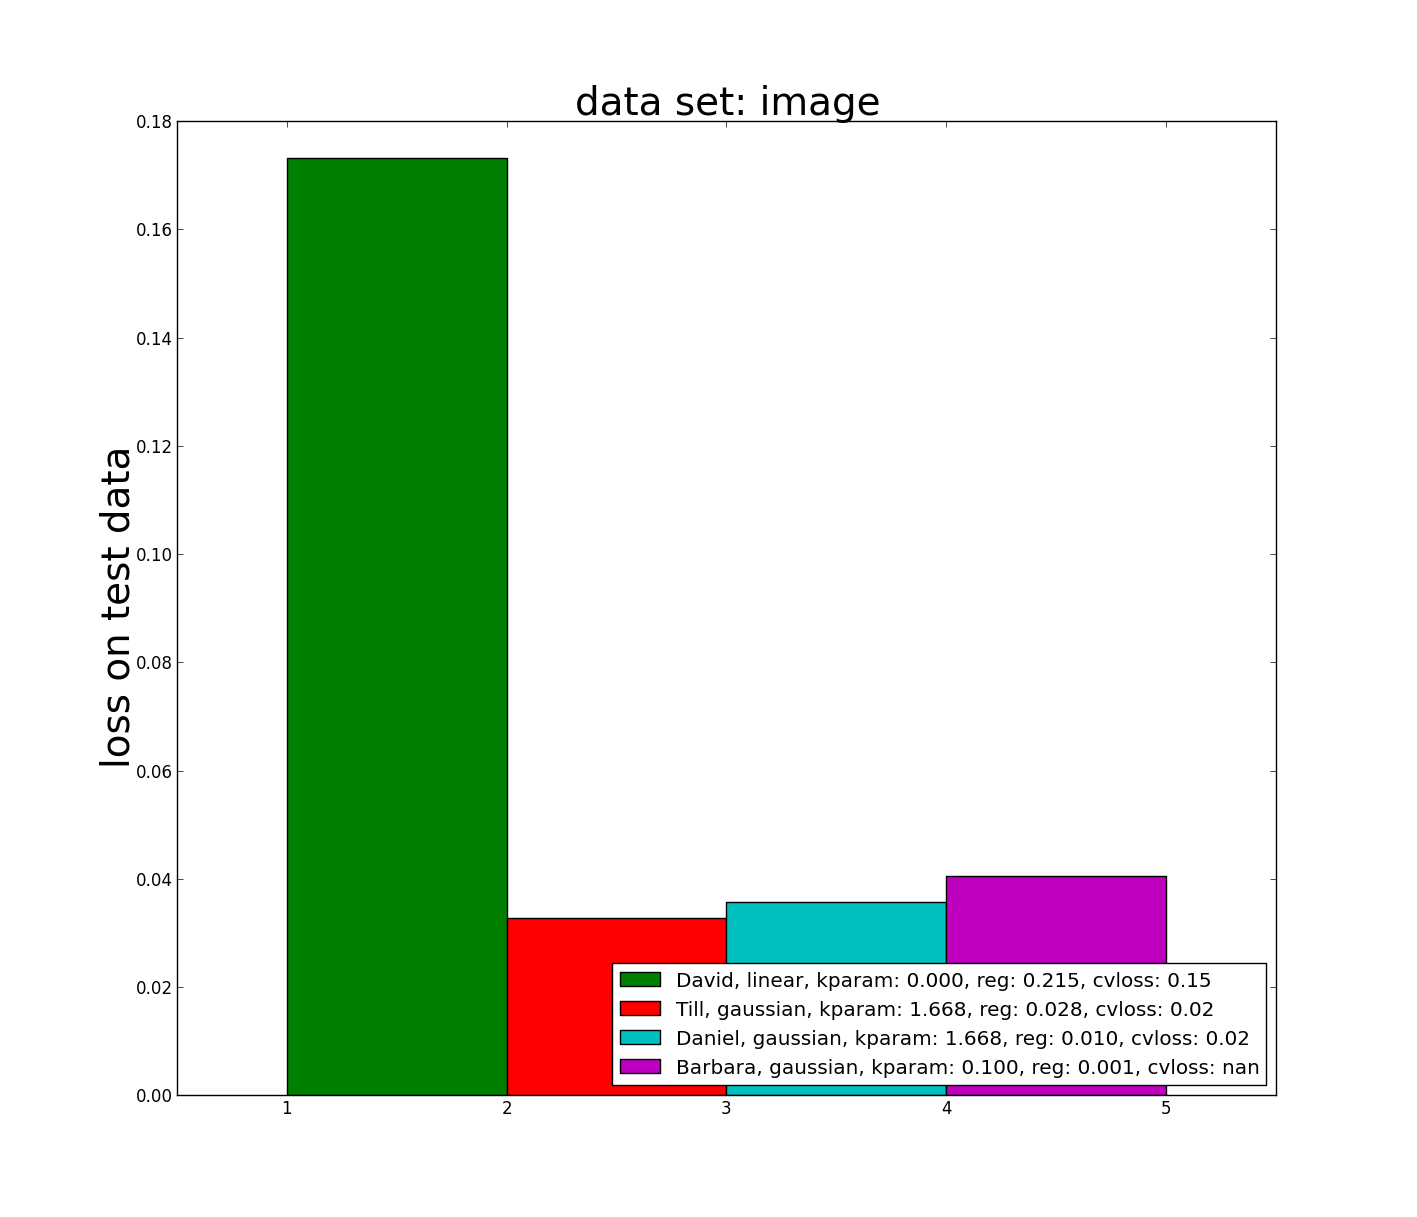
\includegraphics[width=5.75cm]{images/ps3_results_image.png}
	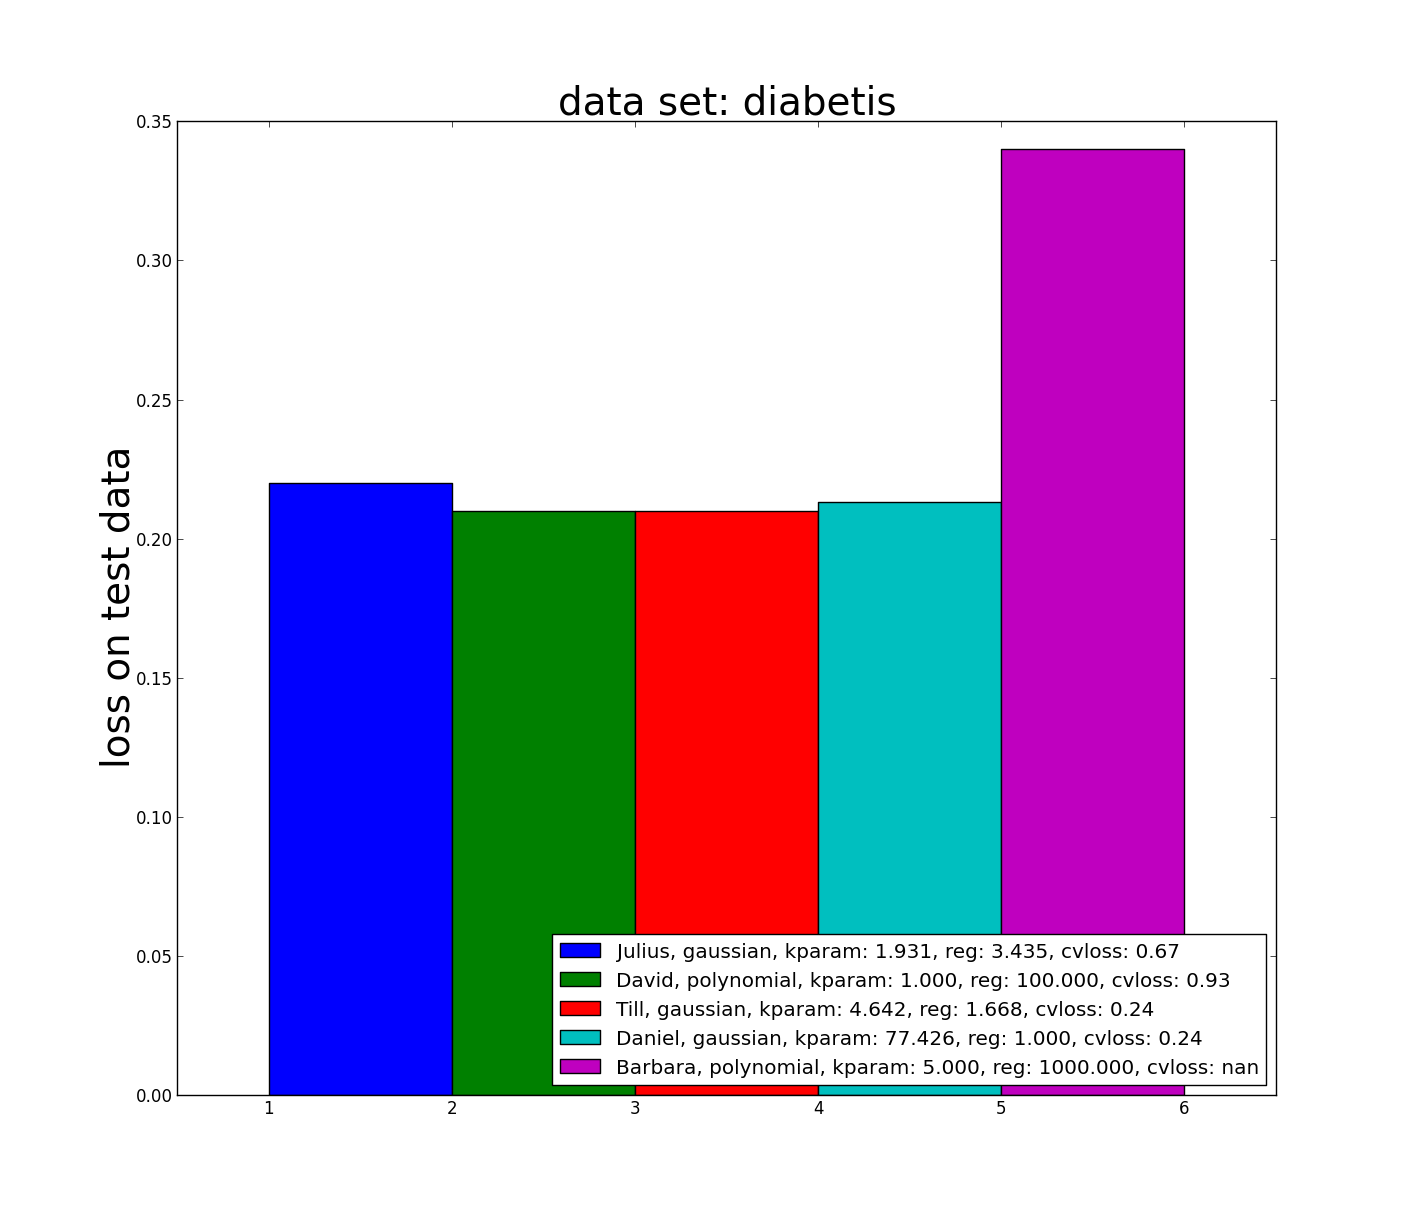
\includegraphics[width=5.75cm]{images/ps3_results_diabetis.png}
\end{frame}

\begin{frame}
	\frametitle{Comparison test data set contd.}
	\begin{center}
		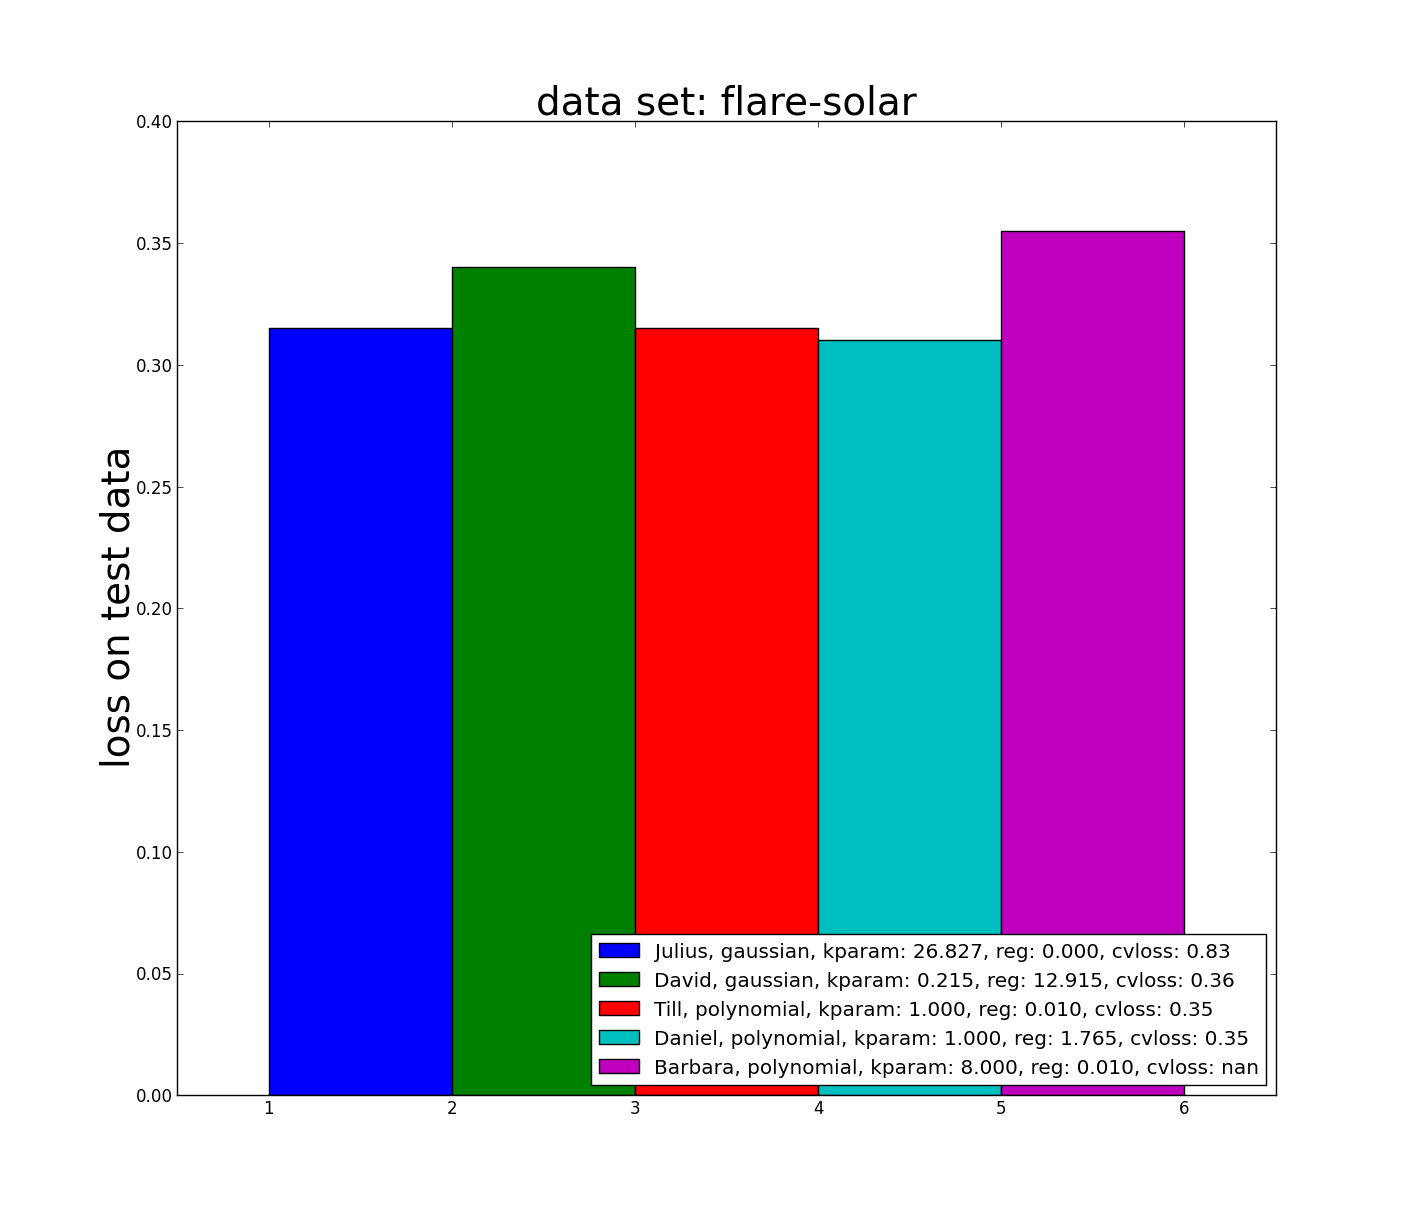
\includegraphics[width=5.75cm]{images/ps3_results_flare-solar.png}
	\end{center}
\end{frame}
